\chapter{State-of-the-art and Brief Literature}
\label{chap:thatchapter}

The teleoperation systems are structurally very interesting and equally challenging systems also from a system theoretical view. As an example, if we isolate the local and the remote devices that would be used to manipulate a distant object or explore a distant environment, we see that they are, whether linear or nonlinear, simple motion-control systems with well-studied properties. Hence, one can view the open-loop teleoperation system as a system with block diagonal structure. 

However, unlike the usual motion-control systems, their exogenous inputs and outputs are coupled with the to-be-designed controller and it is this controller that makes a teleoperation system perform adequately or drive to instability. Moreover, in case of free-air motion, the human force input to the local device should be tracked by the remote device but in case of a hard-contact of remote device with the environment, its effect should be attenuated unilaterally and once again should also be tracked if the local device position reference is pointing away from the obstacle. 



=========== Not good! Better wording!

\section{A Brief Historical Overview}

The inception of the bilateral teleoperation technology is commonly attributed to the work 
of Raymond Goertz in Argonne National Laboratories \cite{goertz} (In \cite{basanezsuarez}, 
it's even traced back to Nikola Tesla). The main motivation of Goertz' work (similarly later in Europe 
by Vertut \cite{vertutcoiffet}) was handling and manipulating nuclear material, hence the very 
first teleoperators are purely mechanical to cope with the hostile environment. Though not much 
happened in terms of realization of devices, the concept of telemanipulation kept its appeal 
and a large body of research was reported until the 1980s. In that decade, with the help of the 
ever-increasing computational power and the popularity of Virtual Reality (VR), teleoperation 
technology received more attention for a possible use in the space-,underwater-,medical-related tasks. We refer 
the reader to \cite{burdea} for a detailed account of these developments 

There is a plethora of choices when it comes to modeling a teleoperation system. 


\begin{figure}%
%http://chat.stackexchange.com/transcript/message/4857161#4857161
\centering
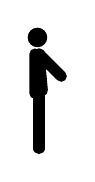
\begin{tikzpicture}[scale=1,manstyle/.style={line width=4pt,line cap=round,line join=round}]
\node[fill,circle,inner sep=2.5pt,outer sep=1pt] at (-0.2mm,7.1mm) {};
\draw[manstyle] (0,0.5) -- ++(0,-1.2cm);
\draw[manstyle] (-1.5pt,0) -- ++(0,0.5cm) (1.2pt,1pt) --(0,5mm)--++(-45:4mm);
\end{tikzpicture}
\caption{General Teleoperation System}%
\label{fig:teleop}%
\end{figure}

The main tool that one has is the physical-interaction-based approach. Hence the view of the designer is tuned to see the energy interaction between two distant media. This approach treats the human and the environment as sources pumping energy to the system and the controller is viewed as the energy regulator preventing excess energy causing the system go unstable. 